\RequirePackage{luatex85}
\documentclass{standalone}
\usepackage{tikz}
\usetikzlibrary{decorations}
\usetikzlibrary{decorations.pathmorphing}
\usetikzlibrary{arrows.meta}
\tikzset{>=latex, line width=1.0pt}
\usepackage{amsmath}
\usepackage{mathtools}
\newcommand{\ct}{\hspace{2pt}\rule[1pt]{3pt}{3pt}\hspace{2pt}}
\DeclareMathOperator{\pr}{pr}
\DeclareMathOperator{\transport}{transport}
\begin{document}
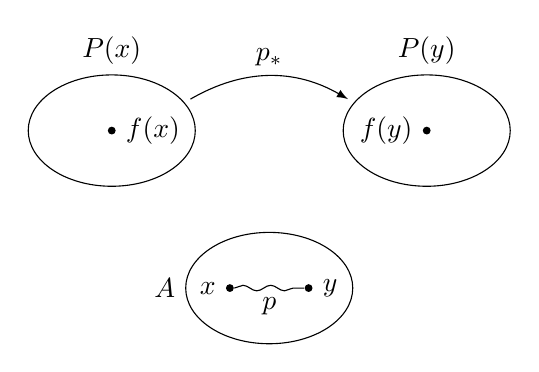
\begin{tikzpicture}
  \def\xshift{2}
  \def\yheight{2}

  % P(x)
  \node[circle,draw,inner sep=0.5cm,label=above:{$P(x)$},xscale=1.5] (px) at (-\xshift,\yheight) {};
  \node[circle,fill,inner sep=1pt,label=right:{$f(x)$}] (b1) at (px) {};

  % P(y)
  \node[circle,draw,inner sep=0.5cm,label=above:{$P(y)$},xscale=1.5] (py) at (\xshift,\yheight) {};
  \node[circle,fill,inner sep=1pt,label=left:{$f(y)$}] (b1) at (py) {};

  % Base space A
  \node[circle,draw,inner sep=0.5cm,label=left:{$A$},xscale=1.5] (A) at (0,0) {};
  \node[circle,fill,inner sep=1pt,label=left:{$x$}] (b1) at (-.5,0) {};
  \node[circle,fill,inner sep=1pt,label=right:{$y$}] (b2) at (.5,0) {};
  \draw[decorate,decoration={snake,amplitude=1}] (b1) -- node[auto,swap] {$p$} (b2);

  \draw[->] (-0.5*\xshift,\yheight+0.2*\yheight) to[bend left] node[auto] {$p_\ast$} (0.5*\xshift,\yheight+0.2*\yheight);
  % \draw[decorate,decoration={snake,amplitude=1}] (b1) -- node[auto] {$f(p)$} (b2);
\end{tikzpicture}
\end{document}